\documentclass[11pt]{article}
\usepackage[margin=1in]{geometry}
\usepackage{booktabs}
\usepackage{amsmath}
\usepackage{amssymb}
\usepackage{graphicx}
\usepackage{hyperref}
\hypersetup{colorlinks=true, linkcolor=blue, urlcolor=blue}
\sloppy

\title{What Predicts Delay, and What Does Not:\\
\large Elapsed hearing time at the San Francisco Planning Commission, 1998--2026}
\author{Dan Post}
\date{September 2026}

\begin{document}
\maketitle

\begin{abstract}
\noindent
A case the Commission hears more than once is a project it did not finish with. This memo asks
how much of the elapsed time between a case's first hearing and its last can be forecast from
what a developer could observe on the day of that first hearing: the kind of request, the
staff recommendation published beforehand, the zoning district, the supervisor district, the
year, the turnout at the hearing.

\medskip\noindent
The answer is: the level, somewhat; the tail, barely. Everything observable together explains
\textbf{17.0\% of the variance} of $\log(\text{days}+1)$ in sample and \textbf{9.6\% out of
sample}, forecasting cases first heard from 2016 with a model fitted only on cases through
2015. For the events that actually hurt --- more than a year from first hearing to last ---
the same covariates reach \textbf{$R^2=0.055$ in sample and $0.032$ out of sample}. Sorting
every case into deciles of predicted delay, the worst decile still finishes within a year
\textbf{95\% of the time}, and the best decile fails to \textbf{1.2\%} of the time. The model
separates expected delay across deciles by a factor of a hundred and separates tail risk by a
factor of four.

\medskip\noindent
The residual is the finding. Conditional on returning at all, the residual standard deviation
is 1.06 log points --- realised delay is routinely a factor of three away from its predicted
value --- and within the \emph{best-informed} decile of returning cases the 10th and 90th
percentiles are 28 days and 675 days. That gap, not the mean, is what a project with
financing costs is exposed to, and it is the first available proxy for the cost of
uncertainty this project is ultimately about.

\medskip\noindent
Nothing here is causal. These are descriptive predictive regressions on a chain of hearing
dates, and the memo is careful about what the chain is and is not.
\end{abstract}

\tableofcontents
\newpage

\section{The construction}

Chain the item table by case number --- upper-cased, whitespace stripped --- order by hearing
date, and take the first and last appearance. \textbf{8{,}987 cases} result from the
16{,}199 items, of which \textbf{39.1\% are heard on more than one day} and \textbf{34.1\%
show a positive elapsed time} (Table~\ref{tab:returning}). The gap between those two numbers is cases heard twice at the
same meeting, as sub-items \texttt{1a} and \texttt{1b}, which are one hearing however they are
numbered.

Three things this measure is not, stated once so the rest of the memo can be read against
them.

\textbf{It is not the entitlement clock.} It starts when an item first reaches an agenda,
already well downstream of filing, and it ends at the last hearing rather than at the permit.
The pre-hearing wait --- which the permit-linkage memo shows runs a median 245 days on the
\emph{other} side of the hearing --- is invisible here. This is hearing-to-hearing time and
nothing more.

\textbf{The case number is an imperfect project identifier.} A project that re-files takes a
new case number, and its old chain closes. Two-thirds of cases show no elapsed time at all,
and some of those are projects that came back under a different number. The chains are
therefore a \emph{lower bound} on how often projects return.

\textbf{The corpus is bounded at both ends.} It begins in 1998, so a case first heard that
year may have been running since 1996, and the 1998--2000 archive is thin (about 12 meeting
documents a year against roughly 40 from 2001). It ends 2026-03-26, so a case first heard in
2024 cannot yet show a two-year tail. Every regression in this memo therefore drops cases
first heard within three years of the corpus end, leaving \textbf{8{,}382 cases}; the
descriptive table marks the censored cohorts rather than dropping them.

% GENERATED BY analyze_delay.py — do not edit by hand.
\begin{table}[htbp]\centering
\caption{Elapsed days from first hearing to last, by five-year cohort of first hearing, over all 8{,}987 cases. `Returned' is the share heard on more than one day. Cohorts marked $\dagger$ are right-censored --- the corpus ends 2026-03-26 --- and are shown for completeness only; the regressions drop every case first heard within 3 years of that date.}\label{tab:cohorts}
\begin{tabular}{lrrrrrr}\toprule
First heard & Cases & Returned & Median & 90th pct & 99th pct & Max\\\midrule
1998--1999 & 629 & 47\% & 0 & 77 & 341 & 665\\
2000--2004 & 1,995 & 36\% & 0 & 77 & 416 & 3157\\
2005--2009 & 1,769 & 39\% & 0 & 85 & 475 & 2408\\
2010--2014 & 1,559 & 27\% & 0 & 77 & 518 & 2737\\
2015--2019 & 1,502 & 28\% & 0 & 119 & 798 & 3423\\
2020--2024$^\dagger$ & 1,431 & 29\% & 0 & 84 & 640 & 1316\\
2025--2026$^\dagger$ & 102 & 13\% & 0 & 7 & 56 & 70\\
\bottomrule\end{tabular}\end{table}

\begin{table}[htbp]\centering
\caption{OLS of $\log(\text{days}+1)$ on what is observable at the first hearing, added one block at a time. Estimation sample: cases first heard on or before 2023-03-26. The dependent variable's standard deviation is 1.981.}\label{tab:ladder}
\begin{tabular}{lrrrr}\toprule
Specification & $N$ & $R^2$ & Adj.\ $R^2$ & Residual s.d.\\\midrule
Request type only & 8,382 & 0.045 & 0.043 & 1.937\\
$+$ staff recommendation & 8,382 & 0.121 & 0.118 & 1.860\\
$+$ zoning district & 8,382 & 0.124 & 0.119 & 1.859\\
$+$ supervisor district & 8,382 & 0.129 & 0.123 & 1.855\\
$+$ year of first hearing & 8,382 & 0.143 & 0.134 & 1.843\\
$+$ speakers at first hearing & 8,382 & 0.170 & 0.161 & 1.814\\
$+$ arrived already continued & 8,382 & 0.170 & 0.161 & 1.814\\
\bottomrule\end{tabular}\end{table}

\begin{table}[htbp]\centering
\caption{The full specification on three outcomes. The level is fitted two to three times as well as the tail indicators, and no outcome gets past a fifth of its variance.}\label{tab:tails}
\begin{tabular}{lrrrr}\toprule
Outcome & $N$ & Mean & $R^2$ & Unexplained variance\\\midrule
$\log(\text{days}+1)$ & 8,382 & 1.339 & 0.170 & 83.0\%\\
$\mathbb{1}[\text{days}>180]$ & 8,382 & 0.047 & 0.090 & 91.0\%\\
$\mathbb{1}[\text{days}>365]$ & 8,382 & 0.018 & 0.055 & 94.5\%\\
\bottomrule\end{tabular}\end{table}

\begin{table}[htbp]\centering
\caption{Out of sample. The model is fitted on cases first heard through 2015 and used to forecast cases first heard from 2016 on; year fixed effects are dropped because they cannot extrapolate. One test case is excluded for carrying a category level that never appears in the training years. Out-of-sample $R^2$ is computed against the training mean, so a negative value would mean the model forecasts worse than that constant.}\label{tab:oos}
\begin{tabular}{lrrrrr}\toprule
Outcome & Train $N$ & Test $N$ & In-sample $R^2$ & Out-of-sample $R^2$ & Test mean\\\midrule
$\log(\text{days}+1)$ & 6,155 & 2,226 & 0.176 & 0.096 & 1.298\\
$\mathbb{1}[\text{days}>180]$ & 6,155 & 2,226 & 0.080 & 0.054 & 0.070\\
$\mathbb{1}[\text{days}>365]$ & 6,155 & 2,226 & 0.047 & 0.032 & 0.032\\
\bottomrule\end{tabular}\end{table}

\begin{table}[htbp]\centering
\caption{Quantile regressions of $\log(\text{days}+1)$ on the full specification, conditional on the case returning at all ($N=2862$). Pseudo-$R^2$ does not fall in the upper tail --- the model fits the 90th percentile about as well as the median, in relative terms. What grows is the quantity being fitted.}\label{tab:quantiles}
\begin{tabular}{lrr}\toprule
Quantile & Pseudo-$R^2$ & Unconditional value (days)\\\midrule
$\tau=0.10$ & 0.135 & 8\\
$\tau=0.25$ & 0.108 & 21\\
$\tau=0.50$ & 0.112 & 49\\
$\tau=0.75$ & 0.138 & 105\\
$\tau=0.90$ & 0.158 & 238\\
\bottomrule\end{tabular}\end{table}

\begin{table}[htbp]\centering
\caption{Cases sorted into deciles of predicted delay, against what actually happened. The model separates the deciles by a factor of a hundred in expectation and by a factor of about ten in realised median, but the tail risk in the worst decile is still only one case in twenty.}\label{tab:calibration}
\begin{tabular}{lrrrrrr}\toprule
Decile & Cases & Expected & Median & 75th & 90th & $>$365 d\\\midrule
1 & 839 & 0.2 & 0 & 0 & 21 & 1.2\%\\
2 & 840 & 0.8 & 0 & 0 & 14 & 0.5\%\\
3 & 836 & 1.3 & 0 & 0 & 35 & 1.0\%\\
4 & 841 & 1.7 & 0 & 0 & 35 & 1.0\%\\
5 & 835 & 2.1 & 0 & 0 & 49 & 1.0\%\\
6 & 841 & 2.6 & 0 & 21 & 70 & 1.0\%\\
7 & 835 & 3.3 & 0 & 28 & 98 & 2.0\%\\
8 & 838 & 4.3 & 0 & 35 & 93 & 2.0\%\\
9 & 838 & 7.2 & 7 & 56 & 141 & 3.7\%\\
10 & 839 & 22.5 & 49 & 126 & 266 & 5.0\%\\
\bottomrule\end{tabular}\end{table}

\begin{table}[htbp]\centering
\caption{The same specification on the cases that came back at all. The residual spread, not the fit, is the quantity of interest: a one-standard-deviation surprise multiplies realised delay by 2.9, and inside the decile the model expects to take longest the realised distribution still runs from 28 to 675 days.}\label{tab:returning}
\begin{tabular}{lr}\toprule
Quantity & Value\\\midrule
Cases in the estimation sample & 8,382\\
\quad heard on more than one day & 39.1\%\\
\quad with a positive elapsed time & 34.1\%\\
Cases used here (days $>$ 0) & 2,862\\
$R^2$ & 0.191\\
Dependent-variable s.d.\ (log points) & 1.163\\
\textbf{Residual s.d.\ (log points)} & \textbf{1.063}\\
\quad as a multiplicative factor & 2.9$\times$\\
Top predicted decile ($n=287$): 10th pct & 28 days\\
\quad median & 175 days\\
\quad 90th pct & 675 days\\
\bottomrule\end{tabular}\end{table}

\begin{table}[htbp]\centering
\caption{Delay by the staff recommendation published before the first hearing. It is the single most informative thing a developer can read, and it is public and dated. Categories with fewer than 60 cases omitted.}\label{tab:recommendation}
\begin{tabular}{lrrrr}\toprule
Preliminary recommendation & Cases & Median & 90th pct & $>$365 days\\\midrule
\texttt{other} & 65 & 21 & 452 & 13.8\%\\
\texttt{no\_action} & 327 & 0 & 442 & 12.2\%\\
\texttt{disapprove} & 117 & 7 & 206 & 3.4\%\\
\texttt{pending} & 275 & 35 & 203 & 3.3\%\\
\texttt{uphold\_neg\_dec} & 108 & 32 & 177 & 3.7\%\\
\texttt{initiate} & 98 & 35 & 135 & 0.0\%\\
\texttt{missing} & 1,612 & 0 & 105 & 1.6\%\\
\texttt{took\_dr\_and\_approved} & 347 & 0 & 70 & 0.6\%\\
\texttt{did\_not\_take\_dr} & 1,551 & 0 & 63 & 0.3\%\\
\texttt{took\_dr} & 136 & 0 & 63 & 0.0\%\\
\texttt{approve} & 3,477 & 0 & 49 & 1.5\%\\
\texttt{adopt} & 231 & 0 & 42 & 0.9\%\\
\bottomrule\end{tabular}\end{table}


\section{The stylised facts}

Table~\ref{tab:cohorts} gives elapsed time by five-year cohort of first hearing, over all
cases. Two patterns, and only one of them is about the middle of the distribution.

\textbf{The centre is nearly stable.} Conditional on a case returning at all, the median is
\emph{exactly} 35 days in all four cohorts from 1998 through 2014 --- essentially the
Commission's own meeting cycle, which is what a routine continuance of two or three meetings
costs. It is not perfectly flat: it rises to 63 days for cases first heard 2015--19 and 49 for
2020--24, so the middle of the distribution did move somewhat, and a memo that says otherwise
is overstating the contrast. Unconditionally the median is zero, because two-thirds of cases
are finished the first time they are heard.

\textbf{The tail moved, and it moved a long way.} The unconditional 99th percentile went from
\textbf{341 days} for cases first heard in 1998--99 to \textbf{798 days} for 2015--19. The
90th percentile of cases that returned at all --- reported in the corpus memo --- went from
147 days to 360 over the same span. The share of cases that return did not rise; if anything
it fell, from 47\% to 28\%. Fewer projects come back, and the ones that do come back stay
longer.

That combination is what makes the variance rather than the mean the object of interest. A
developer facing a distribution whose centre has not moved in twenty-five years but whose
upper decile has doubled is facing a worse problem than the median suggests, and cannot
diversify it away over a single project.

\section{What predicts the level}

Table~\ref{tab:ladder} builds the specification one block at a time, on $\log(\text{days}+1)$.
Four things are worth reading off it.

\textbf{The request type alone explains 4.5\%.} A variance is a different animal from a
conditional use, and both differ from a General Plan amendment, but knowing which one you are
is a small part of the answer.

\textbf{The staff recommendation nearly triples that}, to 12.1\%, and it is the single largest
addition anywhere in the ladder. This matters practically because the recommendation is
\emph{published before the hearing} and is populated on 81\% of cases. It is the most
informative thing a developer can read, and they can read it in advance. Section~\ref{sec:rec}
takes it on its own.

\textbf{Geography adds almost nothing.} The zoning district takes $R^2$ from 0.121 to 0.124,
and the supervisor district --- recovered by joining the item's parcel to DBI's permit table,
which carries a district on 99.8\% of its rows --- takes it to 0.129. Where a project is
matters far less to how long it takes than what it is asking for and what staff thinks of it.
This is a mild surprise and it is worth stating, because the natural prior is that some
neighbourhoods are simply harder.

\textbf{Turnout adds 2.7 points, and must not be over-read.} Adding the log speaker count
takes $R^2$ from 0.143 to 0.170, with a coefficient of $-0.356$ ($t=-16.4$): \emph{more}
speakers, \emph{less} delay. That is not a finding about mobilisation. Half of all cases have
no speakers recorded at the first hearing, and 50\% of those were continued at that hearing,
against 14\% of cases that did have speakers. A hearing with no speakers is usually a hearing
that did not happen --- an item rolled to the next calendar without being taken up. The
speaker count is largely a marker of whether the item was substantively heard, and it predicts
delay for that reason.

\textbf{Arriving already continued adds nothing at all.} 7.4\% of cases first appear with the
minutes noting a prior continuance. Its coefficient is $+0.016$ ($t=0.21$) and it moves $R^2$
by less than a thousandth. A case that has already been rolled once is not, conditional on
everything else, a case that will be rolled again.

\section{The tail is a different problem}

\begin{figure}[htbp]\centering
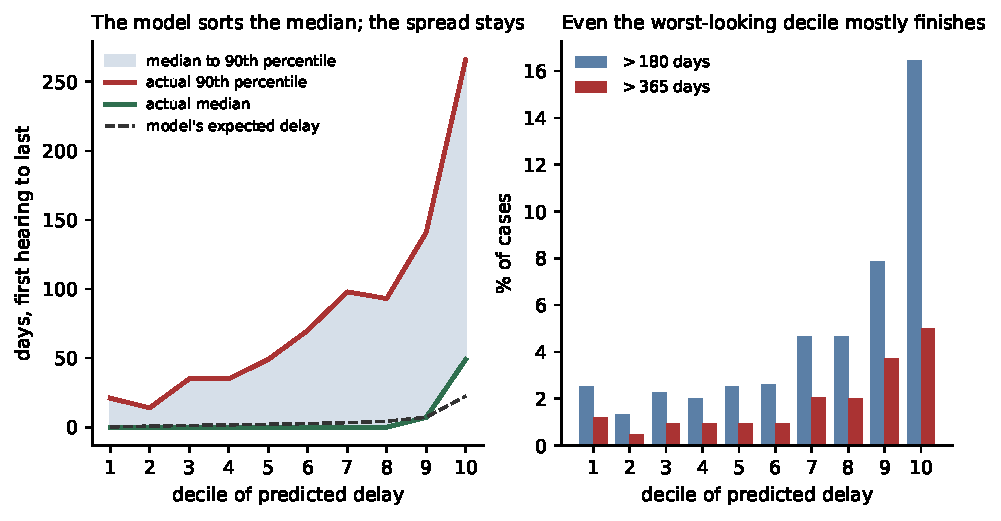
\includegraphics[width=\textwidth]{figures/fig_delay_predictability.pdf}
\caption{Cases sorted into deciles of predicted delay from the full specification. Left: the
model's expected delay against what the decile actually did. Right: realised tail risk by
decile. The model orders the deciles correctly; the distribution inside each of them stays
wide, and the absolute level of tail risk stays low everywhere.}
\label{fig:predictability}
\end{figure}

Table~\ref{tab:tails} runs the full specification on three outcomes. On the level it reaches
$R^2 = 0.170$. On $\mathbb{1}[\text{days}>180]$ it reaches 0.090, and on
$\mathbb{1}[\text{days}>365]$, 0.055. \textbf{Between 83\% and 95\% of the variance is
unexplained}, and the share unexplained rises as the outcome moves into the tail.

Table~\ref{tab:calibration} and Figure~\ref{fig:predictability} are the interpretable version.
Sorting all 8{,}382 cases into deciles of predicted delay:

\begin{itemize}
\item The model's \emph{expected} delay runs from 0.2 days in the first decile to 22.4 in the
tenth --- a factor of a hundred, so the model is doing real work in ordering cases.
\item The \emph{realised} median runs from 0 to 49 days, and the realised 90th percentile from
21 to 266.
\item But the probability of running past a year runs only from \textbf{1.2\% to 5.1\%}. The
worst-looking tenth of the docket, on everything a developer can see, still finishes within a
year nineteen times out of twenty.
\end{itemize}

So the observables sort cases, but they do not identify the cases that will go badly wrong.
The tail is not concentrated in an identifiable part of the docket; it is spread thinly across
all of it. For a developer, that is worse than if it were concentrated: a project cannot avoid
the risk by not being the kind of project that attracts it.

Table~\ref{tab:quantiles} adds quantile regressions on the cases that returned at all, and
this is where an initial hypothesis has to be corrected. The natural guess is that the
covariates fit the median and fail in the tail. In relative terms they do not: pseudo-$R^2$ is
0.111 at the median and \emph{rises} to 0.156 at the 90th percentile. The model fits the upper
quantile about as well as the middle one. What changes is the scale of what is being fitted.
The unconditional 90th percentile is 238 days against a median of 49; explaining 16\% of a
large number still leaves a large number. The failure is not one of relative fit but of
absolute residual spread, and \S\ref{sec:residual} puts a number on it.

\section{Out of sample}

$R^2$ computed on the sample the model was fitted to is an upper bound on what anyone could
actually have forecast. Table~\ref{tab:oos} therefore fits on cases first heard through 2015
and forecasts cases first heard from 2016 on, dropping year fixed effects because a model
containing them cannot say anything about a year it has not seen.

\textbf{The level: 0.176 in sample, 0.096 out.} Roughly half the apparent fit does not
survive. \textbf{More than 180 days: 0.080 in, 0.054 out. More than 365 days: 0.047 in, 0.032
out.} All three out-of-sample numbers are positive, so the model does beat forecasting every
case at the historical mean --- but a developer applying the historical relationship to a new
project would have accounted for about one tenth of the variation in how long it took, and
about one thirtieth of whether it ran past a year.

The gap between in-sample and out-of-sample fit is itself informative: it means the
relationship between observables and delay is not stable across the period. That is consistent
with the pattern the corpus memo documents --- a Commission that moved from denial to
conditioning and from single hearings to repeat ones, at different rates for different kinds
of request.

\section{The staff recommendation as a prior}
\label{sec:rec}

\begin{figure}[htbp]\centering
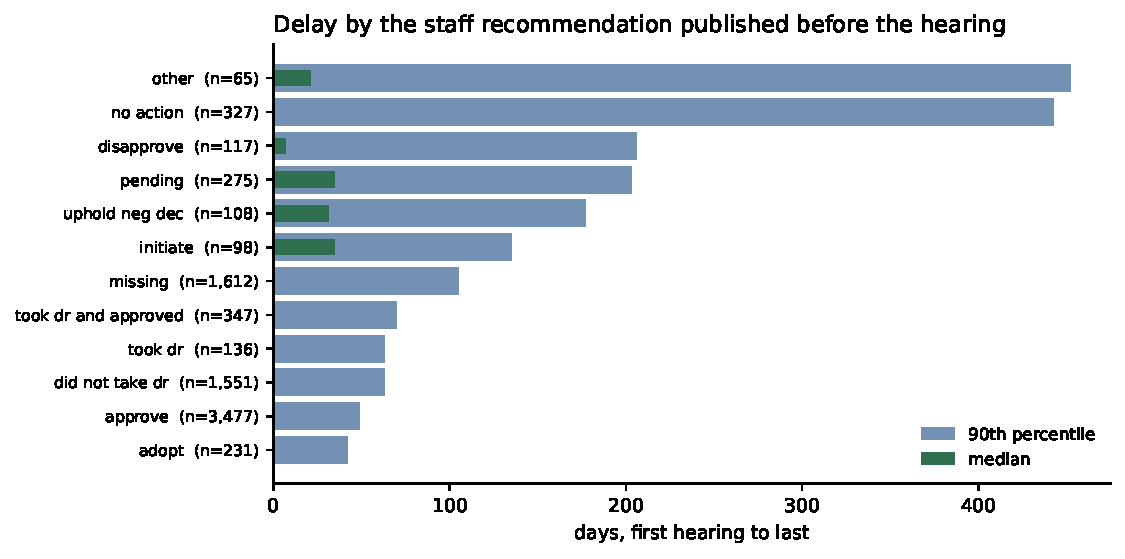
\includegraphics[width=\textwidth]{figures/fig_delay_recommendation.pdf}
\caption{Median and 90th-percentile elapsed time by the preliminary recommendation published
before the first hearing, for categories with at least 60 cases.}
\label{fig:recommendation}
\end{figure}

Table~\ref{tab:recommendation} cuts delay by the preliminary recommendation. This is the one
covariate with an unambiguous \emph{ex ante} interpretation: it is issued by staff, published
in the packet before the hearing, and available on 81\% of cases.

The spread is large. A case where staff recommended \texttt{approve} --- 3{,}477 cases, the
largest group by far --- has a median of 0 days, a 90th percentile of 49, and a 1.5\% chance
of running past a year. A case marked \texttt{no\_action} has a 90th percentile of 442 days
and a \textbf{12.2\%} chance of running past a year: eight times the risk. \texttt{Pending}
and \texttt{disapprove} sit in between, at 3.3\% and 3.4\%.

Two readings, and they are not exclusive. Staff may be forecasting: they see the file, know
what is unresolved, and the recommendation encodes it. Or the recommendation may be
constituting the outcome: a case staff will not recommend is a case the Commission will not
approve on the day. Separating those requires variation in the recommendation that is not a
function of the project, which this design does not have. Either way, as a \emph{signal} it
works, and it is free and public.

Two cautions. \texttt{no\_action} and \texttt{other} are small and heterogeneous categories,
and \texttt{missing} --- 1{,}612 cases, a fifth of the sample --- has a 90th percentile of 105
days, above \texttt{approve} and below everything else, so the missingness is not ignorable.
And what the brief called ``departure from staff'' cannot be tested here: whether the
Commission departed from the recommendation is known only after the hearing, so it is an
outcome, not a predictor.

\section{The residual as a proxy for the cost of uncertainty}
\label{sec:residual}

The fitted value is expected delay conditional on observables. The residual is the part no one
could have forecast, and it is the object the paper is ultimately about.

Over all cases, the residual standard deviation is \textbf{1.814 log points}
(Table~\ref{tab:ladder}) against a dependent-variable standard deviation of 1.981. That figure
is inflated by the mass point at zero, so the cleaner statement conditions on the case
returning at all. Table~\ref{tab:returning} reports it: there $R^2 = 0.191$ and the
\textbf{residual standard deviation is 1.063 log points}, meaning a one-standard-deviation
surprise multiplies realised delay by about \textbf{2.9}.

The sharpest version is inside the top decile. Among the 2{,}862 cases that returned, the 287
in the decile the model expects to take longest have a 10th percentile of \textbf{28 days}, a
median of 175 and a 90th percentile of \textbf{675 days} --- a twenty-four-fold spread among
projects that look identical on every observable. A developer who has read the staff report, knows the zoning, knows the request
type and can see the room is still facing that.

This is a proxy and it should be labelled as one. It is a residual from a descriptive
regression, not a structural estimate of a subjective distribution, and it inherits every
limitation in \S1: it measures hearing-to-hearing time on a lower-bound chain, over a docket
selected by having reached a hearing at all. What it does establish is an order of magnitude.
Whatever the option value of waiting is worth in this market, it is being priced against a
distribution whose conditional spread is a factor of twenty, not a factor of two.

\section{What would sharpen this}

\begin{enumerate}
\item \textbf{Start the clock earlier.} DataSF's Planning Records carry \texttt{open\_date} for
the case, which is the filing date. Joining it would turn hearing-to-hearing time into
filing-to-decision time and make the pre-hearing wait --- currently invisible --- part of the
measure.
\item \textbf{Follow the chain past the hearing.} The permit-linkage memo establishes that for
matched items the permit's issuance date is observable, a median 245 days after the hearing.
Total time from first hearing to permit is constructible today for the discretionary-review
part of the docket.
\item \textbf{Fix the identifier.} Case-number chains break when a project re-files. The
parcel is a stable key, and linking chains that share a parcel within a few years would raise
the measured return rate and lengthen the measured tail. Both directions push the same way:
the numbers here are conservative.
\item \textbf{Model the tail directly.} A linear probability model on a 1.8\% event is a blunt
instrument. A duration model with competing risks --- approved, withdrawn, still pending ---
would use the shape of the hazard rather than a threshold, and would handle the censoring the
current design side-steps by dropping cases.
\item \textbf{Condition on the conditions.} Whether a case that was going to be conditioned
heavily takes longer is not testable while \texttt{conditions\_imposed} is a yes/no flag. The
conditions memo sets out what recovering the content would take.
\end{enumerate}

\section{Reproducing this}

\texttt{code/commission\_minutes\_processing/analyze\_delay.py} produces every number, table
and figure here. It reuses \texttt{chains()} from \texttt{analyze\_corpus.py} rather than
re-deriving the panel, joins DBI for the supervisor district through
\texttt{analyze\_permits.py}, and reads \texttt{labels.db} only for the ``arrived already
continued'' flag, degrading gracefully to \texttt{False} if that local store is absent. No
number in this memo is hand-placed.

\end{document}
